\chapter{Proposta de Solução}
\label{cap:proposta}

A solução proposta para permitir a realização de experimentos de plataformas de Cidades Inteligentes em ambientes simulados abrangendo diferentes cenários em diferentes escalas será
apresentada neste capítulo.
A discussão sobre os requisitos de uma possível solução para esse problema se dará de maneira genérica, contudo, ao abordarmos a arquitetura, entraremos em alguns detalhes referentes ao
simulador de Cidades Inteligentes InterSCSimulator e a plataforma InterSCity, as ferramentas utilizadas neste trabalho.
Além disso, serão apresentados alguns exemplos de implementação de cenários de Cidades Inteligentes seguindo a arquitetura proposta, trazendo em seguida os principais problemas e
dificuldades encontradas nesse processo.

\section{Requisitos da Solução}
\label{sec:requisitos}

Para a realização de experimentos em ambientes simulados de Cidades Inteligentes temos requisitos em diferentes níveis, desde a capacidade do simulador de representar o contexto
de uma cidade até formas de comunicação que permita a interação entre o simulador e a plataforma de Cidades Inteligentes.
Portanto, dividimos os requisitos em \textbf{fundamentais} e de \textbf{integração}.

Para que o simulador possa refletir o contexto de Cidades Inteligentes, onde o sensoriamento de diversos aspectos das cidades já é uma realidade, e a atuação (modificação do estado
das cidades) segue uma crescente, consideramos que a mesma deva ter de alguma forma representada os conceitos abaixo:

\begin{itemize}
    \item \textit{Modelos aderentes a realidade de uma cidade}: o simulador deve implementar modelos que representem ao máximo a realidade de uma cidade, e não apenas casos hipotéticos.
        Por exemplo, modelos de fluxo de automóveis nas vias devem incluir possíveis engarrafamentos.

    \item \textit{Execução com noção de tempo real}: a dinâmica da cidade deve ser simulada em tempo real, ou seja, não deve ser executada nem mais rápida nem mais lenta do que aconteceria
        em um ambiente real de uma cidade (um segundo simulado é aproximadamente igual a um segundo real).
        Esse é um requisito importante, pois o desencadeamento de ações nas cidades são muitas vezes devido ao processamento de ações acontecidas anteriormente, e as plataformas
        devem ter tempo hábil para realizar tais ações, como foi explicado nos capítulos anteriores.

    \item \textit{Geração de grande massa de dados}: para realizarmos experimentos realistas devemos ser capazes de gerar uma massa de dados na mesma escala de uma grande cidade por
        exemplo.
        Experimentos em escalas menores são úteis na validação de certos cenários, contudo não exercita uma plataforma de Cidades Inteligentes em um contexto real, onde deverá
        interagir com milhões de sensores, atuadores e usuários.

    \item \textit{Comunicação em tempo de execução}: para que esse ambiente integrado seja viável, ambas as ferramentas devem ser capazes de se comunicarem em tempo de execução.
        Com isso, se torna possível a envio de dados de sensores e comandos de atuação durante a emulação.
\end{itemize}

Consideramos os pontos apresentados acima como \textbf{requisitos fundamentais}, sendo esses o mínimo necessário para conseguirmos de fato representar um ambiente real de uma cidade.
Caso a ferramenta atenda os requisitos apresentados, se torna possível a simulação de cenários realistas no contexto de Cidades Inteligentes, podendo substituir \textit{testbeds}
reais, em uma escala maior, após a sua integração com a plataforma alvo.
Todavia, apenas essa simulação não viabiliza ainda a realização de experimentos com plataformas, ainda precisamos atender alguns \textbf{requisitos de integração} entre o simulador
e a plataforma em questão.

Para termos um ambiente integrado precisamos definir um meio de comunicação de duas vias, envio e recebimento de dados, em tempo real entre o simulador e a plataforma de Cidades Inteligentes.
Além disso, deve haver uma integração semântica que viabilize as ferramentas se comunicarem de maneira eficaz.
Abaixo são apresentados os \textbf{requisitos de integração} necessários para obtermos um ambiente integrado de experimentação para essas plataformas:

\begin{itemize}
    \item \textit{Integração semântica}: para que seja possível a comunicação em tempo de execução entre o simulador e a plataforma, ambos precisam entrar em um consenso semântico.
        Abaixo são apresentados os dois principais conceitos envolvidos e que acreditamos que seja necessário serem representados de alguma forma em ambas as ferramentas para que seja
        possível a integração.

        \begin{itemize}
            \item \textit{Recursos da cidade}: esse recursos da cidade, sendo eles qualquer coisa no contexto da cidade (automóveis, aparelhos públicos, vias e etc.), serão objetos tanto de
                sensoriamento e/ou atuação por parte das plataformas de Cidades Inteligentes.

            \item \textit{Capacidades inerentes a cada recurso da cidade}: cada \textit{recurso da cidade} tem as suas respectivas capacidades, sendo elas de sensoriamento ou atuação.
                Essas capacidades usualmente estão atreladas a dispositivos heterogêneos de IoT (\textit{Internet Of Things}) presentes nos recursos da cidade.
                Por exemplo, vagas de estacionamento podem ser monitoradas quanto a sua ocupação, e semáforos de trânsito podem ter o seu estado modificado através de atuação.
        \end{itemize}

    \item \textit{Envio de dados de sensoriamento em tempo real}: para que as funcionalidades relativas a coleta e armazenamento de dados, e processamento dos mesmos possam ser
        exercitadas pela plataforma, precisamos enviar dados de todos os recursos presentes no cenário de experimentação com tais capacidades em tempo real.
        Quanto maior for a escala do cenário de experimentação mais difícil se torna essa tarefa, pois se faz necessário enviar milhões de dados de sensores simultaneamente através
        do mesmo canal.
        Apesar de a demanda de tempo real poder se tornar um problema, ela se faz necessária para que possamos chegar mais próximo de um cenário realista, onde recursos sensoriados
        da cidade poderão não aguardar outros enviarem seus dados para enviar, apenas enviarão no tempo estipulado.

    \item \textit{Recebimento de dados de atução em tempo real}: as plataformas, em dados cenários de experimentação, precisarão enviar comandos de atuação para a cidade (neste caso,
        para o ambiente simulado) em tempo real.
        Diferente dos dados de sensoriamento, o fluxo de dados de atuação é bem menor.
        Contudo, esse tipo de dado tem a sua própria peculiaridade, pois o simulador deve ser capaz de consumir esse dado em tempo de execução e alterar o estado do ambiente simulado
        imediatamente.
        Isso porque ao modificar de alguma forma o estado do ambiente simulado influenciamos diretamente os dados de sensores naquele dado momento em diante, e os mesmos continuam
        sendo enviados para a plataforma em paralelo.
\end{itemize}

Portanto, acreditamos que ao termos um ambiente que atenda tanto os \textbf{requisitos fundamentais} quanto os de \textbf{integração}, se torna possível realizarmos experimentos
com plataformas de Cidades Inteligentes sem a necessidade de \textit{testbeds} reais.
Isso nos possibilita testar cenários em escalas reais de uma cidade, além de nos permitir simular cenários que ainda não são passíveis de reprodução através de \textit{testbeds},
simulando tecnologias ainda não existentes e cenários futuristas.
Por exemplo, termos a possibilidade de emular um ambiente onde todos os carros da cidade são autônomos se comunicando através de tecnologia \textit{5G}.

\section{Arquitetura}

Uma arquitetura de software foi desenhada visando atender principalmente os \textbf{requisitos de integração} para construção de um ambiente simulado de experimentação para plataformas
de Cidades Inteligentes, e será apresentada nesta seção.
A integração entre sistemas como apresentando no decorrer deste trabalho é uma tarefa complexa e demanda um projeto de software bem elaborado para que seja manutenível a longo prazo.
Neste trabalho integramos o simulador InterSCSimulator e a plataforma InterSCity para Cidades Inteligents, por isso, ambos serão detalhados quanto a sua respectiva arquitetura na
sequência, além de discutir como os \textbf{requisitos fundamentais e de integração} apresentados serão atendidos em cada ferramenta.

\subsection{Integração Simulador-Plataforma}

A integração entre simulador e plataforma de Cidades Inteligentes envolve principalmete a troca de dados em tempo de execução como foi apresentado neste capítulo.
Essa interação para envio e recebimento de dados a primeira vista simples, se torna complexa quando adicionamos a necessidade de resposta de ambas as partes em tempo real.
Por parte do simulador, a rápida reação ao receber um dado de atuação é essencial.
O recebimento desse dado acarretará em uma atualização no estado da simulação, que por sua vez terá impacto direto no pronto envio de dados de sensores que, por muitas vezes,
se dá de maneira temporizada.
Já para a plataforma, é necessária uma tomada de decisão ágil ao receber diferentes dados de sensores.
Os dados de sensores podem ser, por exemplo, utilizados como entrada para gatilhos de comandos de atuação e processamento em tempo real de eventos complexos.

Além desse desafio, enfrentamos também problemas de interoperabilidade entre o simulador e a plataforma.
Usualmente, os conceitos presentes no projeto de cada uma das ferramentas divergem, e essa camada de integração deve ser capaz de traduzir essa semântica para ambas as ferramentas.
Outro problema relacionado a interoperabilidade é a forma de transmissão desses dados, mais especificamente os protocolos de comunicação a serem utilizados.
Por exemplo, o simulador pode suportar apenas comunicação via protocolo AMQP e a plataforma prover uma API Restful e conexões via MQTT.
Mais uma vez, é papel da camada de integração tornar esse comunicação transparente para ambos os lados.

Tendo isso em vista, a arquitetura de integração adotada utiliza-se de um componente extra intermediando as duas ferramentas, simulador e plataforma, como pode ser visto na
Figura \ref{fig:general_architecture}.
Apesar de um componente extra adicionar complexidade e consequentemente aumentar o tempo gasto na transação desses dados, ele se faz necessário para solucionar os problemas
de interoperabilidade mencionados anteriormente.
Entretanto, ele deve ser o mais simples possível para que o acréscimo no tempo de envio e recebimento dos dados não aumente consideravelmente.
Portanto, utilizar ferramentas (simulador e plataforma) que se assemelhem conceitualmente e que compartilhem pilhas de protocolos de comunicação similares é o ideal,
facilitando o implementação de um ambiente integrado em conformidade com os requisitos apresentados inicialmente.

\begin{figure}[ht]
	\centering
	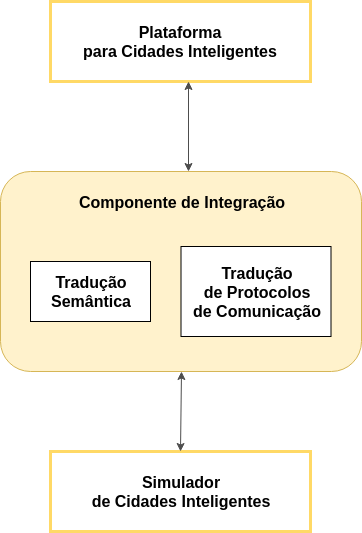
\includegraphics[width=0.4\textwidth]{figuras/integration-general-architecture.png}
	\caption{Arquitetura Proposta para Ambiente Integrado de Exerimentação de Plataformas de Cidades Inteligentes}
	\label{fig:general_architecture}
\end{figure}


Na Figura \ref{fig:general_architecture}, podemos ver os componentes presentes na arquitetura de integração do sistema aqui apresentada.
Como elucidado anteriormente, o componente de integração não pode possuir muitas responsabilidades, já que uma complexidade alta pode acarretar em um aumento expressivo no
tempo de transmissão dos dados, sendo esse um requisito importante para o sistema.
Já as ferramentas envolvidas, além de suas próprias funcionalidades, esperamos que as mesmas possuam um módulo de comunicação para suportar o fluxo de dados em tempo de execução.

O componente de integração tem a responsabilidade de solucionar os pontos mencionados anteriormente:

\begin{itemize}
    \item Tradução semântica entre o simulador e a plataforma

    \item Interoperação entre protocolos de rede

    \item Interferência mínima no tempo de envio e recebimento de dados
\end{itemize}

Como pode ser visto, o componente de integração tem como único objetivo atender requisitos não funcionais.
Ele deve tornar a comunicação do simulador e da plataforma transparente para ambos e adicionando a menor complexidade possível ao sistema.

Em resumo, devemos escolher ferramentas (simulador e plataforma) mais semelhantes possíveis, com o que diz respeito principalmente ao modelo conceitual e aos protocolos de
rede utilizados para comunicação; e implementar o componente de integração o mais simples possível, apenas com o objetivo de viabilizar a comunicação entre as ferramentas.

Para a validação da construção desse ambiente simulado de experimentação para plataformas de Cidades Inteligentes, usamos o simulador InterSCSimulator e a plataforma InterSCity,
sendo essas ferramentas desenvolvidas pelo nosso grupo de pesquisa. Ambas serão apresentadas a seguir, correlacionando os requisitos e a aquitetura de integração aqui
apresentada.

\subsection{InterSCSimulator}

O InterSCSimulator é um simulador de código aberto baseado em agentes para Cidades Inteligentes que oferece uma interface simples para definição de
cenários de larga escala \cite{santana_17}.
Pelo fato de ser possível configurar o tempo que dura um ciclo de simulação na ferramenta, ela já atende um dos \textbf{requisitos fundamentais}.
Com isso, podemos dizer que um ciclo de simulação é igual a um segundo real.
Como apresentado anteriormente, é necessário termos uma execução com noção de tempo real (um segundo de simulação igual a aproximadamente um segundo real) e permitir a
interferência em tempo de execução por terceiros para a construção desse ambiente integrado de experimentação.

Para atingir a escalabilidade mencionada, o InterSCSimulator foi implementado usando a linguagem \textit{Erlang}.
Essa é uma linguagem funcional que visa facilitar a implementação de aplicações de larga escala, paralelas e distribuídas.
Algumas características herdadas do modelo de atores, que é implementado pelo \textit{Erlang}, são: paralelismo, execução distribuída, tolerância a falhas e
protocolo de comunicação \cite{santana_17}.
Essa escalabilidade é importante para que possamos atender o \textbf{requisito fundamental} que diz respeito a capacidade de geração de grandes massas de dados
para a plataforma.
O InterSCSimulator é capaz de simular cenários com milhões de agentes executando simultaneamente, sendo assim possível simular cenários em uma escala realista para cidades de grande porte.

O InterSCSimulator foi implementado por Eduardo Zambom Santana, doutorando de nosso grupo de pesquisa, baseado no simulador de âmbito geral \textit{Sim-Diasca}.
A Figura \ref{fig:simulator_architecture} apresenta a sua arquitetura, onde, em azul, estão os diferentes tipos de agentes que podem existir no ambiente
simulado e, em vermelho, a definição dos cenários de Cidades Inteligentes, tudo isso sendo executado no topo do simulador \textit{Sim-Diasca}.

\begin{figure}[ht]
	\centering
	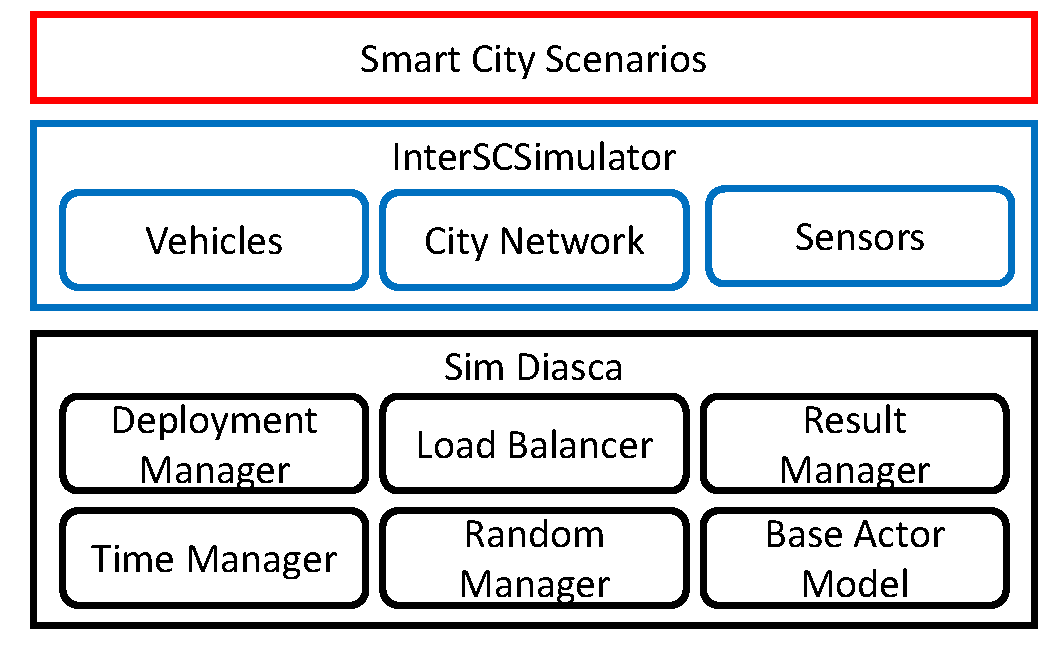
\includegraphics[width=0.5\textwidth]{figuras/Arquitetura.pdf}
	\caption{Arquitetura do InterSCSimulator}
	\label{fig:simulator_architecture}
\end{figure}

Fazendo um paralelo com um dos \textbf{requisito de integração} listados neste capítulo, cada \textit{Recurso} da cidade pode ser modelado como um agente da simulação.
Ou seja, um carro, uma vaga de estacionamento ou um ponto de parada de ônibus serão representados como agentes (caixas azuis na Figura \ref{fig:simulator_architecture})
na arquitetura do InterSCSimulator.
Na definição desses agentes especificamos o seu comportamento a cada passo da simulação.
Com isso, podemos especificar quais as \textit{Capacidades} de cada agente e adotar modelos aderentes com a realidade das cidades modernas.
O interessante dessa arquitetura baseada em agentes é o fato da implementação dos mesmos terem um grau de independência muito grande, onde é preciso apenas a definição
das mensagens que serão trocadas em tempo de execução.

Além disso, no contexto deste trabalho, foi adicionado um novo elemento a arquitetura da ferramenta para troca de dados com sistemas externos em tempo de execução,
sendo esse um dos \textbf{requisitos fundamentais e de integração} para obtermos um ambiente realista de experimentação.
Esse novo elemento nada mais é do que um novo agente onde o seu papel é receber e enviar mensagens de sensores e atuadores, seja no contexto de outros agentes ou de
outros sistemas.

Na implementação de um agente do InterSCSimulator podemos definir diversos comportamentos em diferentes momentos do seu cliclo de vida.
Podemos especificar o que será feito durante a sua criação, a sua destruição, a sua primeira ação na simulação e durante cada ciclo de execução.
Com isso, condições e caminhos dependentes do estado da simulação podem ser definidos para cada um dos tipos de agentes, flexibilizando a implementação dos
mais diversos modelos e formas de prover suas capacidades.
Essa liberdade para implementação de diversos comportamentos dos agentes nos permite usar modelos realistas e viabilizar as capacidades dos recursos no contexto das cidades,
atendendo mais um \textbf{requisito fundamental} e outro de \textbf{integração}.
Por exemplo, um carro após a sua partida em direção ao seu destino, calcula a cada ciclo de execução o fluxo de carros na via em que se encontra para o cálculo da
sua velocidade naquele instante, além de publicar a seu atual posição.
Nesse caso, podemos utilizar os mais diversos modelos matemáticos para calcular o fluxo de carros ou para determinar a sua velocidade, ao passo que a sua capacidade
de publicar sua localização georreferenciada também é atendida.

Na Figura \ref{fig:simulator_components}, são apresentados os componentes do simulador.
Inicialmente são passadas entradas para a simulação (arquivos XML) que em conjunto formam o cenário a ser simulado, esse cenário é executado e a
saída é criada com todos os eventos ocorridos na simulação.
A partir dessa saída existe a possibilidade de geração de uma visualização em um mapa ou através de gráficos.

\begin{figure}[ht]
	\centering
	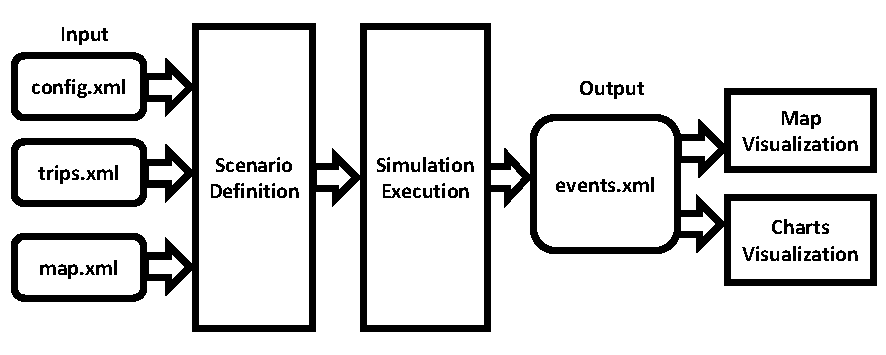
\includegraphics[width=0.7\textwidth]{figuras/Components.pdf}
	\caption{Componentes do InterSCSimulator}
	\label{fig:simulator_components}
\end{figure}

Como entrada, o InterSCSimulator recebe três arquivos XML. O \textit{config.xml} contém parâmetros da simulação, sendo eles o tempo total, o formato do
arquivo de saída e o caminho para o diretório contendo os outros arquivos de entrada e para geração do arquivo de saída.
O grafo representando a infraestrutura rodoviária da cidade é descrito no arquivo \textit{map.xml}, nesse grafo as vias são correspondentes as arestas e as esquinas entre
duas ou mais vias aos nós.
E por fim, as viagens a serem executadas são especificadas no arquivo \textit{trips.xml}, cada viagem contendo o seu tempo de início, modo de transporte, origem e destino.
Todas as ações realizadas pelos agentes são salvos no arquivo \textit{output.xml}, podendo haver quatro ações possíveis: 1) início de viagem, 2) saída de uma via,
3) entrada em uma via, e 4) chegada ao destino final.
O tempo, a localização e o modo de transporte utilizado pelo agente são registrados quando essas ações são salvas.

No trabalho desenvolvido por Eduardo Zambom Santana foi desenvolvido um simulador de larga escala, que é capaz de simular mais de 4 milhões de
agentes se movendo pela cidade de São Paulo~\cite{santana_17}.
Os modos de transportes suportados até então são: carro, ônibus, metrô e a pé.
Neste trabalho além de melhorias feitas nos modelos existentes, novos agentes foram adicionados ao simulador, além de agora ser possível a publicação e recebimento de
eventos em tempo de execução de maneira assícrona.

\subsection{Plataforma InterSCity}
\label{sec:interscity}

A plataforma InterSCity é um projeto de código aberto, baseado em microsserviços que visa permitir a pesquisa colaborativa, desenvolvimento e experimentos em Cidades
Inteligentes~\cite{arthur_17}.
A plataforma foi desenvolvida baseada em uma arquitetura de referência para plataformas de Cidades Inteligentes~\cite{santana_2016}, ela provê um conjunto de serviços
alto-nível baseado em nuvem para gerenciar recursos de \textit{IoT} heterogêneos~\cite{arthur_17}.

O projeto InterSCity visa atacar dois dos principais problemas arquiteturais no desenvolvimento de uma plataforma de alta qualidade que possa ser usada na prática no
contexto de Cidades Inteligentes: escalabilidade e evolução do software~\cite{arthur_17}.
Escalabilidade é necessária pelo fato da plataforma ter que interagir com um grande número de dispositivos \textit{IoT} espalhados pela cidade, milhões de usuários e
um grande tráfego de dados.
Como as cidades mudam constantemente, a questão da evolução é essencial, já que requisitos podem surgir ou mudar a qualquer momento, e adaptar a plataforma a fim de
incorporar novas funcionalidades não deve ser um empecilho.
Para resolver esses dois problemas apresentados, foram adotadas as seguintes estratégias~\cite{arthur_17}:

\begin{itemize}
	\item Modularidade via microsserviços
	\item Modelos e dados distribuídos
	\item Evolução descentralizada
	\item Reuso de projetos de software livre
	\item Adoção de padrões abertos
	\item Comunicação síncrona e assíncrona
	\item Serviços livres de estado
\end{itemize}

A Figura \ref{fig:platform_architecture} apresenta a arquitetura da plataforma InterSCSity.
Atualmente, ela é composta de 6 microsserviços:
\textit{Resource Adaptor}, oferece uma abstração para comunicação com os dispositivos \textit{IoT};
\textit{Data Collector}, responsável por coletar os dados dos sensores conectados;
\textit{Actuator Controller}, oferece uma interface para atuação junto aos dispositivos de \textit{IoT} com tais capacidades;
\textit{Resource Catalog}, possui dados estáticos dos recursos da cidade cadastrados;
\textit{Resource Discovery}, provê um serviço de descoberta de recursos;
e \textit{Resource Viewer}, disponibiliza uma visualização simples dos recursos da cidade. 

\begin{figure}[ht]
	\centering
	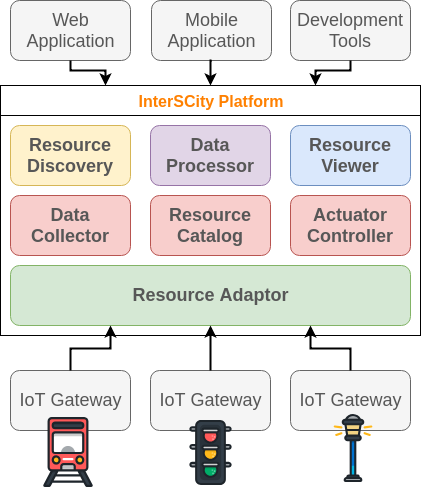
\includegraphics[width=0.5\textwidth]{figuras/platform_architecture.png}
	\caption{Arquitetura da plataforma InterSCity}
	\label{fig:platform_architecture}
\end{figure}

A comunicação entre esses microsserviços pode se dar de maneira síncrona ou assíncrona dependendo da situação.
A comunicação síncrona é feita via API \textit{Restful}, ou seja, requisições HTTP; e a assíncrona se dá via RabbitMQ\footnote{https://www.rabbitmq.com/}, uma implementação do protocolo AMQP.
O objetivo do protocolo AMQP é criar um padrão aberto para troca de mensagens assíncronas interoperável e de larga escala~\cite{vinoski_2006}.
A principal vantagem desse protocolo é permitir que o \textit{broker} de mensagens tome as decisões de roteamento, não necessitando a aplicação ter conhecimento
desse processo~\cite{vinoski_2006}.

A plataforma traz uma abstração chamada \textit{Resource}, que representa um recurso real da cidade, como ônibus, hospital, paradas de ônibus.
Cada um desses \textit{Resources} possuem \textit{Capabilities}, que pode ser de sensoriamento ou atuação, usualmente vinculados a algum tipo dispositivo \textit{IoT},
como capacidade de medir temperatura ou capacidade de mudar o estado de um semáforo.
Esses conceitos são os mesmos apresentados como requisitos para a construção de um ambiente integrado de experimentação para Cidades Inteligentes.
Como apresentado na seção anterior, semânticamente, esses recursos e capacidades aqui apresentados estarão associados a agentes e a definição de ações durante o seu
ciclo de vida no InterSCSimulator.

Na seção a seguir serão apresentados alguns exemplos de implementação da arquitetura aqui proposta utilizando o simulador InterSCSimulator e a plataforma InterSCity
para Cidades Inteligentes.

\section{Exemplos de Implementação}

Com o intuito de validar a arquitetura proposta foram implementados dois cenários de Cidades Inteligentes no ambiente integrado de experimentação.
Priorizamos implementar cenários de experimentação onde pudéssemos explorar todos os requisitos apresentados neste capítulo.

No primeiro cenário realizamos experimentos no contexto de estacionamento inteligente (conhecido com \textit{Smart Parking}), onde carros circulam pela cidade e ao
final do seu percurso procuram por uma vaga de estacionamento disponível mais próxima do seu destino, utilizando-se da plataforma para isso.
Nesse cenário, incluímos um novo agente à simulação e implementamos um mecanismo para publicação dos eventos ocorridos e requisição a serviços da plataforma em tempo real
e de forma assíncrona.

O segundo cenário de experimentação envolve o tráfego de carros inteligente através da utilização de Placas de Mensagens Variadas (PMVs) espalhadas pela cidade.
Nesse cenário a plataforma identifica trechos de maior trânsito e atua na cidade atualizando as mensagens apresentadas pelas PMVs em tempo real, notificando os
motoristas da lentidão no trecho, que por sua vez podem recalcular a sua rota evitando congestionamentos.
Para viabilizar esse experimento nos utilizamos das melhorias implementados no primeiro cenário, modificamos o modelo de trânsito para melhor se adequar a realidade e
implementamos o mecanismo de recebimento de comandos de atuação em tempo de execução.

Cada um desses cenários serão apresentados nas seções a seguir, de maneira a exemplificar a implementação da arquitetura proposta através da utilização do simulador
InterSCSimulator a a plataforma InterSCity para Cidades Inteligentes.

\subsection{Estacionamento Inteligente}
\label{sec:smart_parking}

Como foi apresentado, neste cenário de experimentação, simulamos motoristas realizando seus respoectivos percursos de carro e ao final procurando uma vaga disponível mais próxima ao
seu destino, provavelmente utilizando um aplicativo móvel que se comunica com a plataforma InterSCity.
Trazendo os conceitos de recursos da cidade e capacidades para esse cenário, temos os carros e as vagas de estacionamento sendo recursos, onde os carros são capazes de
fornecer a sua geolocalização (por exemplo via GPS) e as vagas de fornecer informação quanto a sua disponibilidade (por exemplo através de sensores infravermelho e uma
redes de sensores).

Esse cenário foi definido com o intuito de realizar experimentos envolvendo o serviço de descoberta de recursos da plataforma InterSCity.
Portanto, o aplicativo enviaria a posição do carro naquele momento, o seu destino final e o raio de busca, e a plataforma traria uma lista de vagas de estacionamento
disponíveis mais próximas.
Já no InterSCSimulator, foi necessário realizar algumas melhorias para que os \textbf{requisitos fundamentais} fossem atendidos.
Um novo agente para gerenciar as vagas de estacionamento da cidade, chamado \textit{Parking Controller}, foi implementado.
Esse agente possui a responsabilidade de gerenciar e armazenar dados referentes as vagas de estacionamento, e fazer a interface de comunicação com o componente de
integração que será apresentado mais adiante.
Além disso, modificamos o modelo de viagem do agente \textit{Carro}.
Anteriormente, o \textit{Carro} saia de uma origem e percorriar o seu trajeto até o destino, agora ao chegar próximo do seu destino ele requisita uma vaga disponível mais
próxima e se dirige até a mesma.
Com essas melhorias pudemos simular um cenário que se aproxima da realidade.

Para ilustrar o modelo descrito, a seguir será apresentado o ciclo de execução de um agente \textit{Carro} neste cenário:

\begin{enumerate}
    \item O agente \textit{Carro} é criado

    \item O caminho mais curto entre a origem e o destino é calculado

    \item O agente parte da sua origem no tempo determinado

    \item Ao chegar no nó anterior ao seu destino, uma vaga de estacionamento disponível é requisitada ao agente \textit{Parking Controller}

    \item Ao receber a vaga de estacionamento, o seu trajeto é recalculado em direção a mesma

    \item O agente se direciona e estaciona na vaga de estacionamento descoberta 
\end{enumerate}

Um fluxo alternativo a essa execução seria o carro modificar o seu percurso em direção da vaga de estacionamento (disponível até então), e ao chegar nela outro
carro a ter ocupado antes, sendo esse um caso comum nas grandes cidades.
Nesse caso, outra vaga de estacionamento é requisitada aumentando o seu raio de busca com o intuito de sempre encontrar vagas disponíveis.
Caso o agente do tipo carro necessitar realizar mais de três buscas de vagas disponíveis, o mesmo encerra a sua execução.

Quando o agente \textit{Carro} por fim estaciona em uma vaga disponível, o agente \textit{Parking Controller} é notificado e atualiza a sua estrutura de dados indicando
que a vaga foi ocupada pelo carro.
Além do mais, esse agente é responsável por atualizar o estado da vaga de estacionamento na plataforma.

Agora pensando nos \textbf{requisitos de integração}, o simulador precisa requisitar a plataforma em busca de vagas disponíveis mais próximas, e atualizar o estado
das vagas de estacionamento.
A plataforma InterSCity provê um \textit{API Restful} para comunicação com seus serviços (como o de descoberta de recursos), e o estado dos seus recursos podem ser
atualizados através da própria API ou via protocolo AMQP (\textit{Advanced Message Queuing Protocol}).
Esse levantamento é importante para a tomada de decisão de quais as responsabilidades e como será implementado o componente de integração.
Tendo em vista que a complexidade do componente de integração deve ser a menor possível, e a não existência de um meio de publicação de eventos em tempo de execução
no InterSCSimulator, decidimos utilizar o RabbitMQ (implementação do protocolo AMQP) na implementação desse novo meio de comunicação.
Com isso, o simulador poderia atualizar o estado das vagas diretamente na plataforma de forma assíncrona, sem necessidade de auxílio do componente de integração.
As requisições HTTP feitas ao serviço de descoberta da plataforma seriam feitas pelo componente de integração, principalmente pelo fato de requisições HTTP serem
síncronas, o que poderia travar a simulação na espera por uma resposta.

Para facilitar o entendimento da integração realizada, dividiremos a explicação em duas partes: a primeira visando a requisição de vagas disponíveis mais próximas
do carro ao serviço de descoberta da plataforma InterSCity; e a segunda apresentado o fluxo de atualização do estado de uma vaga de estacionamento (ocupada
ou disponível) baseada na emulação.

A Figura \ref{fig:descoberta} apresenta a integração realizada para utilização do serviço de descoberta provido pela plataforma InterSCity.
O componente de integração foi chamado de \textit{Parking Spot Discoverer}, e foi implementado como um agente Erlang que consegue se comunicar com os agentes da
simulação via troca de mensagens.
O uso do componente de integração se fez necessário para que a simulação exerça a carga que aplicações exerceriam utilizando o protocolo HTTP para acessar
a \textit{API Restful}.
Como dito, requisições HTTP são síncronas, e a realização das mesmas dentro da simulação atrasaria consideravelmente a sua finalização, já que bloquearia a
execução dos agentes enquanto aguardariam a resposta da plataforma.
Antes de chegarmos a tal solução implementamos uma versão onde o próprio simulador realizava requisições HTTP para a plataforma em tempo de execução, entretanto,
essa solução gerou um enorme gargalo.
Descrevemos abaixo o fluxo de atividades apresentado na Figura \ref{fig:descoberta}.

\begin{enumerate}
    \item Ao chegar um nó antes do seu destino, o \textit{Car} solicita a vaga de estacionamento para o agente \textit{Parking Controller}, passando a sua
	localização como parâmetro.

	\item O agente \textit{Parking Controller} então envia a localização para o \textit{Parking Spot Discoverer} que solicita a vaga disponível mais próxima,
	em um raio de 500 metros.

	\item O \textit{Parking Spot Discoverer} faz uma requisição HTTP para o serviço de descoberta da plataforma que retorna a vaga em questão.
	Caso não seja encontrada uma vaga disponível (não ocupada) em um raio de 500 metros, esse raio é multiplicado por dois até que se encontre uma vaga
	disponível.

	\item O identificador da vaga é retornado para o agente \textit{Parking Controller} e ele marca a vaga como utilizada em uma estrutura de dados mantida no simulador.

    \item O identificador da vaga é recebido pelo agente \textit{Car} e a rota é recalculada para chegar até ela.
\end{enumerate}

\begin{figure}[ht]
	\centering
	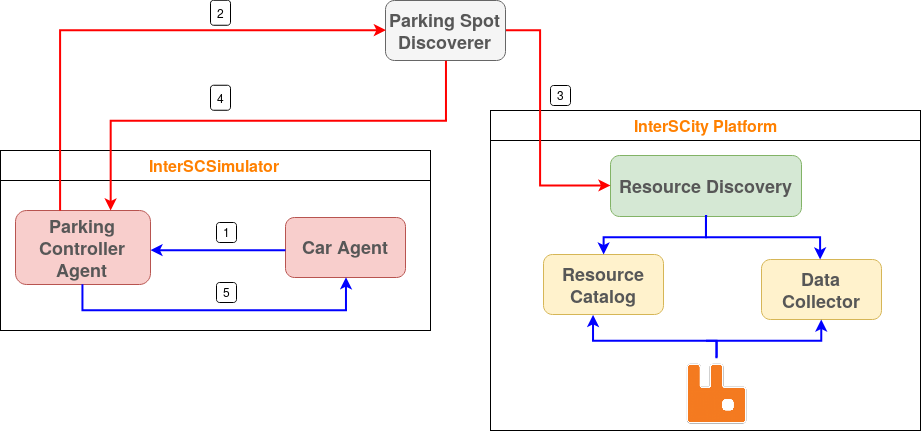
\includegraphics[width=\textwidth]{figuras/integration_get_data_smart_parking.png}
	\caption{Integração para descoberta de vagas livres próximo do destino da
	viagem}
	\label{fig:descoberta}
\end{figure}

A Figura \ref{fig:atualizacao} apresenta a integração realizada com o intuito de atualizar o estado das vagas de estacionamento na plataforma baseado nos
acontecimentos da simulação.
Como foi adicionado a funcionalidade de publicação dos eventos da simulação via RabbitMQ para os interessados, não foi necesário a utilização do
componente de integração, já que a plataforma também utiliza o mesmo protocolo para divulgação dos seus dados entre microsserviços.
O fluxo apresentado na Figura \ref{fig:atualizacao} contém os seguintes passos.

\begin{enumerate}
    \item O agente \textit{Car} estaciona na vaga de estacionamento e notifica o \textit{Parking Controller}.

	\item O \textit{Parking Controller} informa, via \textit{RabbitMQ}, que a vaga está ocupada usando o seu identificador.

	\item O \textit{RabbitMQ} repassa esse dado para os microsserviços \textit{Resource Catalog} e \textit{Data Collector}.
\end{enumerate}

\begin{figure}[ht]
	\centering
	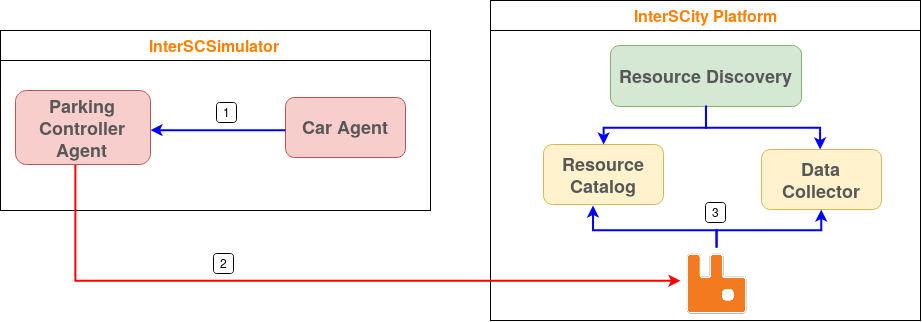
\includegraphics[width=\textwidth]{figuras/integration_publish_data_smart_parking.png}
	\caption{Integração para publicar dados}
	\label{fig:atualizacao}
\end{figure}

Vale ressaltar que as atividades 2 e 3 apresentadas na Figura \ref{fig:atualizacao} também são executadas quando a vaga é liberada.
Após dez minutos que o agente está estacionado na vaga, o agente \textit{Parking Controller} libera a vaga na estrutura de dados mantida dentro do simulador e informa o
ocorrido para a plataforma.
Com isso, a plataforma atualiza os dados da vaga tanto quando ela é ocupada quando liberada.

Após a implementação da arquitetura descrita, fomos capazes de executar experimentos de larga escala no contexto de estacionamento inteligente.
Os resultados obtidos serão apresentados no próximo capítulo.

Todavia, não exercitamos todos os requisitos apresentados para a construção de um ambiente simulado e integrado para experimentação de plataformas de Cidades Inteligentes.
Por isso, implementamos um segundo cenário de Cidades Inteligentes onde, por exemplo, a atuação no ambiente simulado se fez necessária.


\subsection{Tráfego de Carros Inteligente}
\label{sec:smart_traffic}

Com o objetivo de exercitar o envio de comandos de atuação da plataforma para o ambiente simulado, que não foi explorado no cenário de estacionamento inteligente apresentado
anteriormente, definimos um novo cenário.
Neste cenário, visamos identificar trechos em vias da cidade com tráfego de carros anômalo (devido ao fechamento de ruas, acidentes, desastres naturais e etc.) e notificar
previamente os motoristas para evitarem passar naquele trecho através de Placas de Mensagens Variadas (PMVs).
Consideramos aqui uma anomalia uma variação considerável na velocidade média dos carros que trafegam naquele trecho de via naquele horário.
Essas PMVs são posicionadas em pontos estratégicos da cidade e apresentam alertas aos motoristas em tempo real sobre possíveis anomalias no trânsito, e com isso motoristas
podem mudar o seu percurso evitando maiores congestionamentos na cidade.

Essencialmente, esse cenário funciona da seguinte forma:

\begin{enumerate}
    \item A plataforma coleta dados históricos de carros para definir limiares (\textit{thresholds}) de velocidade média para cada trecho de via da cidade em cada horário.
        Para isso, o ambiente simulado envia dados de posicionamento georreferenciado dos carros a cada ciclo de execução, simulando por exemplo um dispositivo que contem um
        sistema de GPRS (\textit{General Packet Radio Service}) + GPS (\textit{Global Positioning System}).
        Com uma série de pontos de onde o carro passou em cada instante, se torna possível calcular a velocidade média do mesmo, logo obtemos a velocidade média de carros
        que passaram naquele trecho naquele dado momento durante todo o dia.
        Tendo esses limiares, a plataforma se torna capaz de identificar anomalias na velocidade média dos carros em tempo real, verificando se a variação naquele instante
        extrapola ou não o que foi identificado com os dados históricos.

    \item Ao identifiar uma anomalia de trânsito em algum trecho, a plataforma identifica as PMVs mais próximas do incidente e atualiza a sua mensagem informando os motoristas
        do ocorrido.

    \item Caso o motorista passe por uma PMV contendo essa mensagem, ele verifica se o trecho mencionado faz parte do seu percurso. Sendo verdade, o mesmo recalcula a sua
        rota evitando maiores congestionamentos na região.
\end{enumerate}

Nesse cenário de experimentação, o novo serviço de processamento de dados (históricos e de tempo real), que está em desenvolvimento, e o envio de comandos de atuação da plataforma
InterSCity puderam também ser testados.
Além disso, foi possível finalizar a validação da arquitetura proposta para a criação de um ambiente para experimentação em plataformas de Cidades Inteligentes,
implementando a atuação em tempo real no ambiente simulado.

Para realizar experimentos envolvendo essas funcionalidades da plataforma InterSCity, foi necessário implementar o conceito de PMVs, eventos de fechamentos de via e de
processamento de comandos de atuação em tempo de execuação no InterSCSimulator.
Além do mais, foi utilizada a publicação de eventos (dados de sensores) implementado para o cenário anterior, já que para o funcionamento do serviço de processamento de dados
em tempo real da plataforma precisamos enviar a cada ciclo de execução da simulação o posicionamento de todos os carros presentes.
Sendo essas melhorias necessárias para atender os \textbf{requisitos fundamentais} para esse cenário.

O modo de publicação de dados em tempo de execução no InterSCSimulator foi refatorado para melhor atender ambos os cenários implementados.
Como visto no cenário anterior, a publicação de eventos da simulação se dava através do agente \textit{Parking Controller} (como pode ser visto na Figura \ref{fig:atualizacao}), já que
até então o único tipo de evento publicado pelo simulador era a atualização da disponibilidade de uma vaga de estacionamento.
No intuito de permitir que outros agentes da simulação também pudessem publicar os seus eventos, um novo agente chamado \textit{Publisher} foi criado, removendo essa responsabilidade
anteriormente atribuída ao agente \textit{Parking Controller}.
Desse modo, o agente do tipo carro também se tornou capaz de publicar a sua posição, onde agora a cada ciclo de execução é enviada uma mensagem a um agente \textit{Publisher}
contendo sua localização.

Visando tornar factível a simulação de eventos de fechamento de vias na cidade, adicionamos o conceito de eventos de trânsito ao InterSCSimulator.
Um novo arquivo de entrada para o simulador e um novo agente foram adicionados.
O novo arquivo de entrada (chamado por padrão \textit{events.xml}), contem uma lista de eventos de fechamento de via que serão agendados na simulação.
Como pode ser visto na Listagem \ref{code:events} abaixo, cada evento é representado da seguinte forma:
(i) o tipo do evento de trânsito;
(ii) a via a ser fechada (uma aresta no grafo da cidade);
(iii) o momento de início do evento;
(iv) a duração do evento;
(v) a porcentagem da capacidade do fluxo de carros que ainda estará em funcionamento, usada no caso de um fechamento parcial do trecho.
O novo agente chamado \textit{Events Manager} é responsável por agendar todos esses eventos no início da simulação e alterar o grafo da cidade no momento programado.
Quando o trecho da via é fechado, a aresta do grafo da cidade é removida momentaneamnte até o evento ser encerrado, impedindo assim a possibilidade de passagem de qualquer
carro.
Agora quando o evento apenas reduz a capacidade de fluxo de carros da via, modificamos a sua capacidade para atender o que foi programado até o evento ser encerrado,
onde essa capacidade é um atributo dado àquela aresta do grafo.

\lstset{
    language=xml,
    tabsize=3,
    frame=lines,
    caption=Arquivo de entrada contendo os eventos de fechamento de vias,
    label=code:events,
    frame=shadowbox,
    rulesepcolor=\color{gray},
    xleftmargin=20pt,
    framexleftmargin=15pt,
    keywordstyle=\color{blue}\bf,
    commentstyle=\color{OliveGreen},
    stringstyle=\color{red},
    numbers=left,
    numberstyle=\tiny,
    numbersep=5pt,
    breaklines=true,
    showstringspaces=false,
    basicstyle=\footnotesize,
    emph={uuid,node},emphstyle={\color{magenta}}}
    \lstinputlisting{files/events.csv}

Para a representação das PMVs no InterSCSimulator, foi criado um agente chamado \textit{PMV Manager} onde o seu papel era atualizar as mensagens de PMVs.
As PMVs em si foram implementadas como atributos de vértices do grafo da cidade (sendo os vértices o encontro de duas ou mais vias), onde nesse atributo é guardada uma lista
de trechos de vias (arestas) onde foram encontradas alguma anomalia no trânsito.
Os agentes do tipo carro ao passar por um vértice que continha esse atributo, verificavam se alguma das arestas ali presentes faziam parte do seu trajeto ou não.
Caso positivo, o seu percurso era recalculado, caso contrário o mesmo se mantinha inalterado.

E a última implementação no InterSCSimulator necessária para atender os requisitos apresentados seguindo a arquitetura proposta foi o recebimento de comandos de atuação e
processamento dos mesmos em tempo de execuação.
Sendo essa uma funcionalidade fundamental para a atualização das PMVs em tempo de execução pela plataforma.
Diante disso, mais um novo agente foi criado para ficar a espera desses comandos enviados pela plataforma, sendo ele chamado de \textit{Listener}.
Como um comando de atuação pode ser enviado a qualquer momento, foi necessário esse novo agente, cuja única responsabilidade é receber esse comando e armazená-lo em uma
estrutura de dados, para que outros agentes não ficassem bloqueados (bloqueando também a simulação) a espera de tal acontecimento.
Ou seja, esse agente fica em um laço (\textit{loop}) infinito a espera de uma mensagem que é enviada via AMQP (mesmo protocolo utilizado para publicação dos dados).
A utilização do RabbitMQ foi escolhida devido a possibilidade da plataforma InterSCity enviar comandos de atuação através do mesmo, e como foi uma funcionalidade nova
decidimos utilizar a mesma tecnologia, reduzindo assim o problema de interoperabilidade discutido neste capítulo.
Quando um comando é recebido, no caso uma aresta de trecho anômalo a ser atualizada em uma PMV, ele armazena essa mensagem em uma estrutura de dados que será acessada no
próximo ciclo de execução pelo \textit{PMV Manager}, que por sua vez atualizará a atributo da referida PMV (vértice no grafo).

Após a apresentação das funcionalidades e melhorias implementadas, as duas vias de fluxo de comunicação entre o simulador e a plataforma serão apresentados a seguir.
Na Figura \ref{fig:smart_traffic_publish_data}, o passo a passo para a publicação dos dados de posicionamento de cada um dos carros a cada ciclo de execução é exposto.

\begin{figure}[ht]
	\centering
	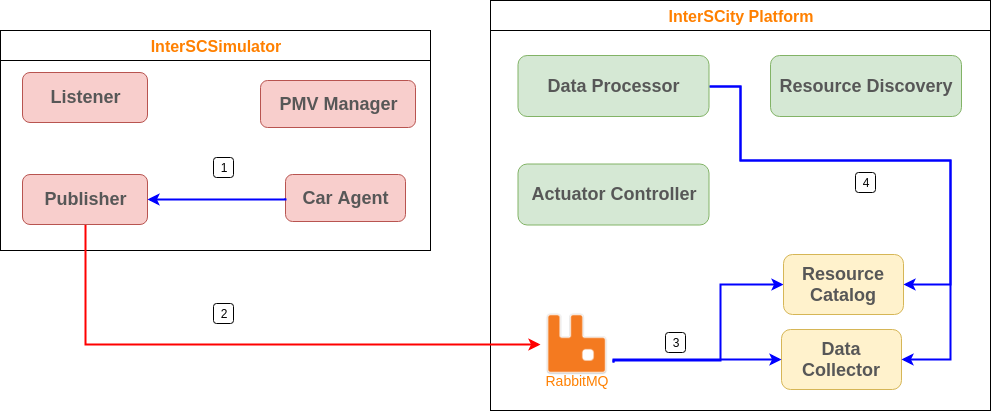
\includegraphics[width=\textwidth]{figuras/integration-publish-car-position.png}
	\caption{Integração para publicar dados de posicionameto de carros}
	\label{fig:smart_traffic_publish_data}
\end{figure}

\begin{enumerate}
    \item O agente do tipo carro a cada ciclo de execução envia uma mensagem para o agente \textit{Publisher} contendo a sua posição naquele dado momento.

    \item O agente \textit{Publisher} se conecta ao \textit{broker} do RabbitMQ e publica uma mensagem contendo: o identificador do carro, o seu posicionamento, e o \textit{timestamp}.

    \item Os microsserviços \textit{Resource Catalog} e \textit{Data Collector} são notificados e recebem tais dados. O \textit{Resource Catalog} atualiza o último dado monitorado
        daquele carro, e o \textit{Data Collector} atualiza a sua base de dados contendo todas as medições.

    \item O microsserviço \textit{Data Processor} acessa dados armazenados por esses outros serviços com o intuito de definir limiares para velocidade média de vias (dados históricos),
        ou para identificar anomalias no trânsito (fluxo de dados em tempo real).
\end{enumerate}

Já na Figura \ref{fig:smart_traffic_actuation}, é apresentado o fluxo para atualização da lista de trechos anômalos de vias em PMVs, representando aqui um comando de atuação no
ambiente simulado.
Lembrando que o gatilho para a execução desse processo é o serviço de processamento de dados identificar alguma anomalia no trânsito.

\begin{figure}[ht]
	\centering
	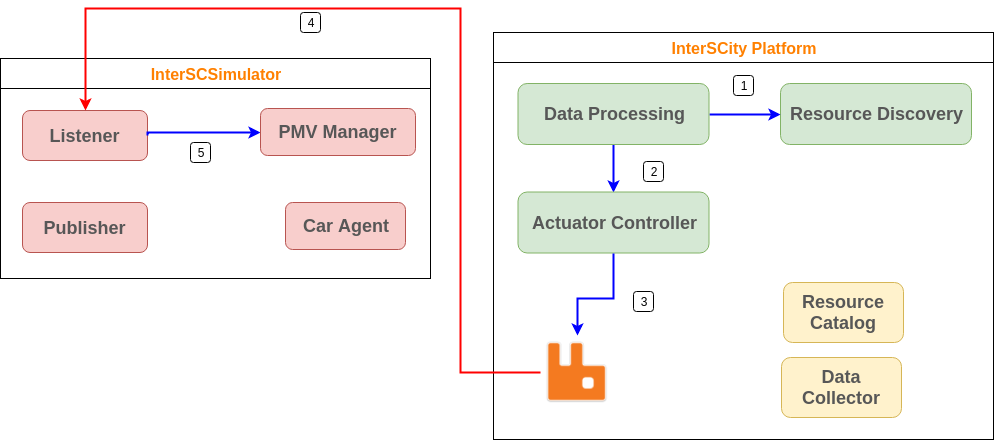
\includegraphics[width=\textwidth]{figuras/integration-actuate-pmv.png}
	\caption{Integração para atuação em Placas de Mensagens Variadas}
	\label{fig:smart_traffic_actuation}
\end{figure}

\begin{enumerate}
    \item O \textit{Data Processor} ao identificar uma anomalia no trânsito em determinado ponto da cidade, ele requisita para o \textit{Resource Discovery} as PMVs mais próximas
        daquele ponto, para que as mesmas possam ser atualizados.

    \item Ao serem identificados as PMVs, o \textit{Data Processor} envia os identificadores das PMVs e do trecho anômalo para o \textit{Actuator Controller}.

    \item O \textit{Actuator Controller} formata essas mensagens e publica as mesmas em um dos canais do RabbitMQ.

    \item O agente \textit{Listener}, cujo único papel é esperar por esse tipo de mensagem, recebe a mesma e a armazena em uma estrutura de dados compatilhada pelos agentes do simulador.

    \item O agente \textit{PMV Manager} verifica a presença dessa nova mensagem na estrutura de dados compatilhada, e atualiza o atributo que representa a PMV no vértice do grafo
        viário da cidade, adicionado mais esse trecho para a lista presente ou criando-a caso não existe nenhum outro trecho.
\end{enumerate}

Um ponto interessante desse segundo cenário, foi a não necessidade de um componente de integração, já que ambas as ferramentas se comunicam através do mesmo protocolo (inclusive a
mesma ferramenta) e conseguem representar os mesmos conceitos de maneira equivalente.
Esse é o cenário ideal para criação de um ambiente simulado de experimentação para uma plataforma de Cidades Inteligentes, já que não foi essencial a implementação desse
componente extra, que como discutido traria mais complexidade para o sistema, podendo aumentar o tempo de resposta entra as ferramentas.
Claro que tudo isso foi possível porque neste mesmo trabalho fizemos toda a implementação dos \textbf{requisitos fundamentais} apresentados, portanto,
tivemos a oportunidade de tomar as decisões técnicas que facilitaram a integração entra as duas ferramentas.

No capítulo a seguir, serão apresentados alguns resultados experimentais baseados na implementação desse cenário de tráfego de carros inteligente.

\section{Discussão}

Durante a implementação dos dois cenários de Cidades Inteligentes apresentados, algumas adversidades foram encontradas e solucionadas.
A fim de contribuir com trabalhos futuros que sigam a solução aqui proposta, uma discussão sobre os principais problemas e dificuldades encontradas será feita
nesta seção.
O intuito aqui é enfatizar os principais obstáculos a serem enfrentados durante a implementação de novos cenários no ambiente integrado usando o simulador InterSCSimulator e
a plataforma InterSCity ou até mesmo envolvendo outras ferramentas.

Como vem sendo discutido no decorrer deste trabalho, a integração de ferramentas não é algo trivial.
Apesar de tanto o simulador quanto a plataforma utilizada serem voltados para o contexto de Cidades Inteligentes, na maioria das vezes, elas não foram concebidas inicialmente
para serem integradas com ferramentas de outra natureza.
Através dos próprios requisitos apresentados podemos antever o maior desafio a ser enfrentado: a interoperabilidade.
Interoperabilidade essa tanto a nível de comunicação e quanto semanticamente.

Como constatado na implementação dos dois cenários apresentados, tentamos ao máximo reduzir a responsabilidade do componente de integração, que ao ser atribuído muitas
tarefas pode se tornar um problema.
Tanto que não foi necessária a implementação desse componente no segundo cenário apresentado, tendo em vista que as ferramentas já atendiam os requisitos de integração.
Isso pode ser atribuído ao fato de ambas as ferramentas (InteSCSimulator e InterSCity) serem mantidas pelo nosso grupo de pesquisa, onde tivemos a liberdade de evoluir o
que foi preciso nas próprias ferramentas para facilitar a integração.
Em um contexto onde não existe essa flexibilidade o desafio se tornario bem mais complexo.

Mesmo assim, enfrentamos problemas principalmente com a escalabilidade da solução.
Em experimentos anteriores e isolados, foi demonstrado que ambas as ferramentas eram escaláveis, se comportando bem diante de uma grande carga de trabalho.
Entretanto, a integração traz alguns elementos extras que por menor que sejam interferem em cenários de larga escala.
Em experimentos na escala de uma cidade como São Paulo, qualquer mínimo detalhe é potencializado.
Semanticamente não tivemos muitos problemas, já que ambas as ferramentas foram implementadas seguindo conceitos similares, devido a própria sinergia do grupo de
pesquisa.
Todavia, a comunicação entre as ferramentas foi a raíz da maior parte dos problemas enfrentados.

Por exemplo, inicialmente, tentamos realizar qualquer interação com a plataforma através de requisições HTTP, usando a sua API \textit{Restful}.
Contudo, percebemos que o componente de integração necessitaria de uma complexidade muito maior para tratar todas essas requisições paralelamente sem se tornar um
gargalo para o sistema.
Por isso, decidimos explorar bastante o protocolo AMQP através da implementação do RabbitMQ.
Essa se apresentou uma solução mais simples, já que o \textit{broker} do RabbitMQ trata todas essas questões de escalabilidade de maneira bem eficiente, sendo essa
uma solução adotada pelo mercado.
Além do mais, pelo fato da comunicação via AMQP ser assíncrona e pela própria natureza dos cenários implementados, diferente de requisições HTTP, ela se apresentou uma
solução mais adequada, não bloqueando agentes da simulação a espera de respostas.
Logo, sempre que possível, transferir responsabilidades para ferramentas de terceiros comprovadamente capazes de atender os requisitos ao invés de implementar a sua
própria solução é desejável.

Nesse processo de melhoria da escalabilidade da solução integrada, várias mudanças foram feitas em ambas as ferramentas.
Foram encontrados problemas de escalabilidade antes não evidenciados por outros experimentos isolados, demonstrado que a solução de ambiente para experimentação para
plataformas de Cidades Inteligentes atingiu seus objetivos, apontando melhorias nos sistemas que só seriam evidenciadas ao enfrentar cargas de trabalho à nível de uma
cidade como São Paulo.

A nível da plataforma InterSCity, implementações envolvendo técnicas para armazenamento em cache de dados mais utilizados foram feitas.
Ademais, melhorias envolvendo a automatização da implantação do plataforma foram realizadas.
Já no InterSCSimulator, encontramos alguns problemas na implementação dos modelos apresentados que causaram problemas de escalabilidade.
Ou seja, dependendo do cenário e de como foi implementado, apenas reduzir a complexidade do componente de integração (até mesmo a não existência) ainda não é a solução.
Portanto, poder modificar as próprias ferramentas é algo interessante, haja vista que a forma que os modelos, métodos e funcionalidades foram implementados podem não
ter sido testados em ambientes de estresse, tornando-se gargalos durante experimentos de larga escala.

Isso evidencia a importância da utilização de ferramentas livres para a construção de ambientes de experimentação para plataformas de Cidades Inteligentes.
